% An example second appendix from the example thesis thesis.tex.
\chapter{EE 518 Test Results}

\section*{E E 518 Lab Tests}

Further testing of the square-law detector was performed by using the radiometer in a real world event.  This test was exercised in conjunction with the Microwave Remote Sensing class (E E 518) under Dr. Brian Hornbuckle.  For this test the radiometer was installed on the roof of Agronomy Hall and was configured so that it could be rotated so it will have a clear view of the sky.  This allowed us to make measurements with a cold source and then at the ground to record a warm source.


{\begin{figure}[h!tb] 
\centering
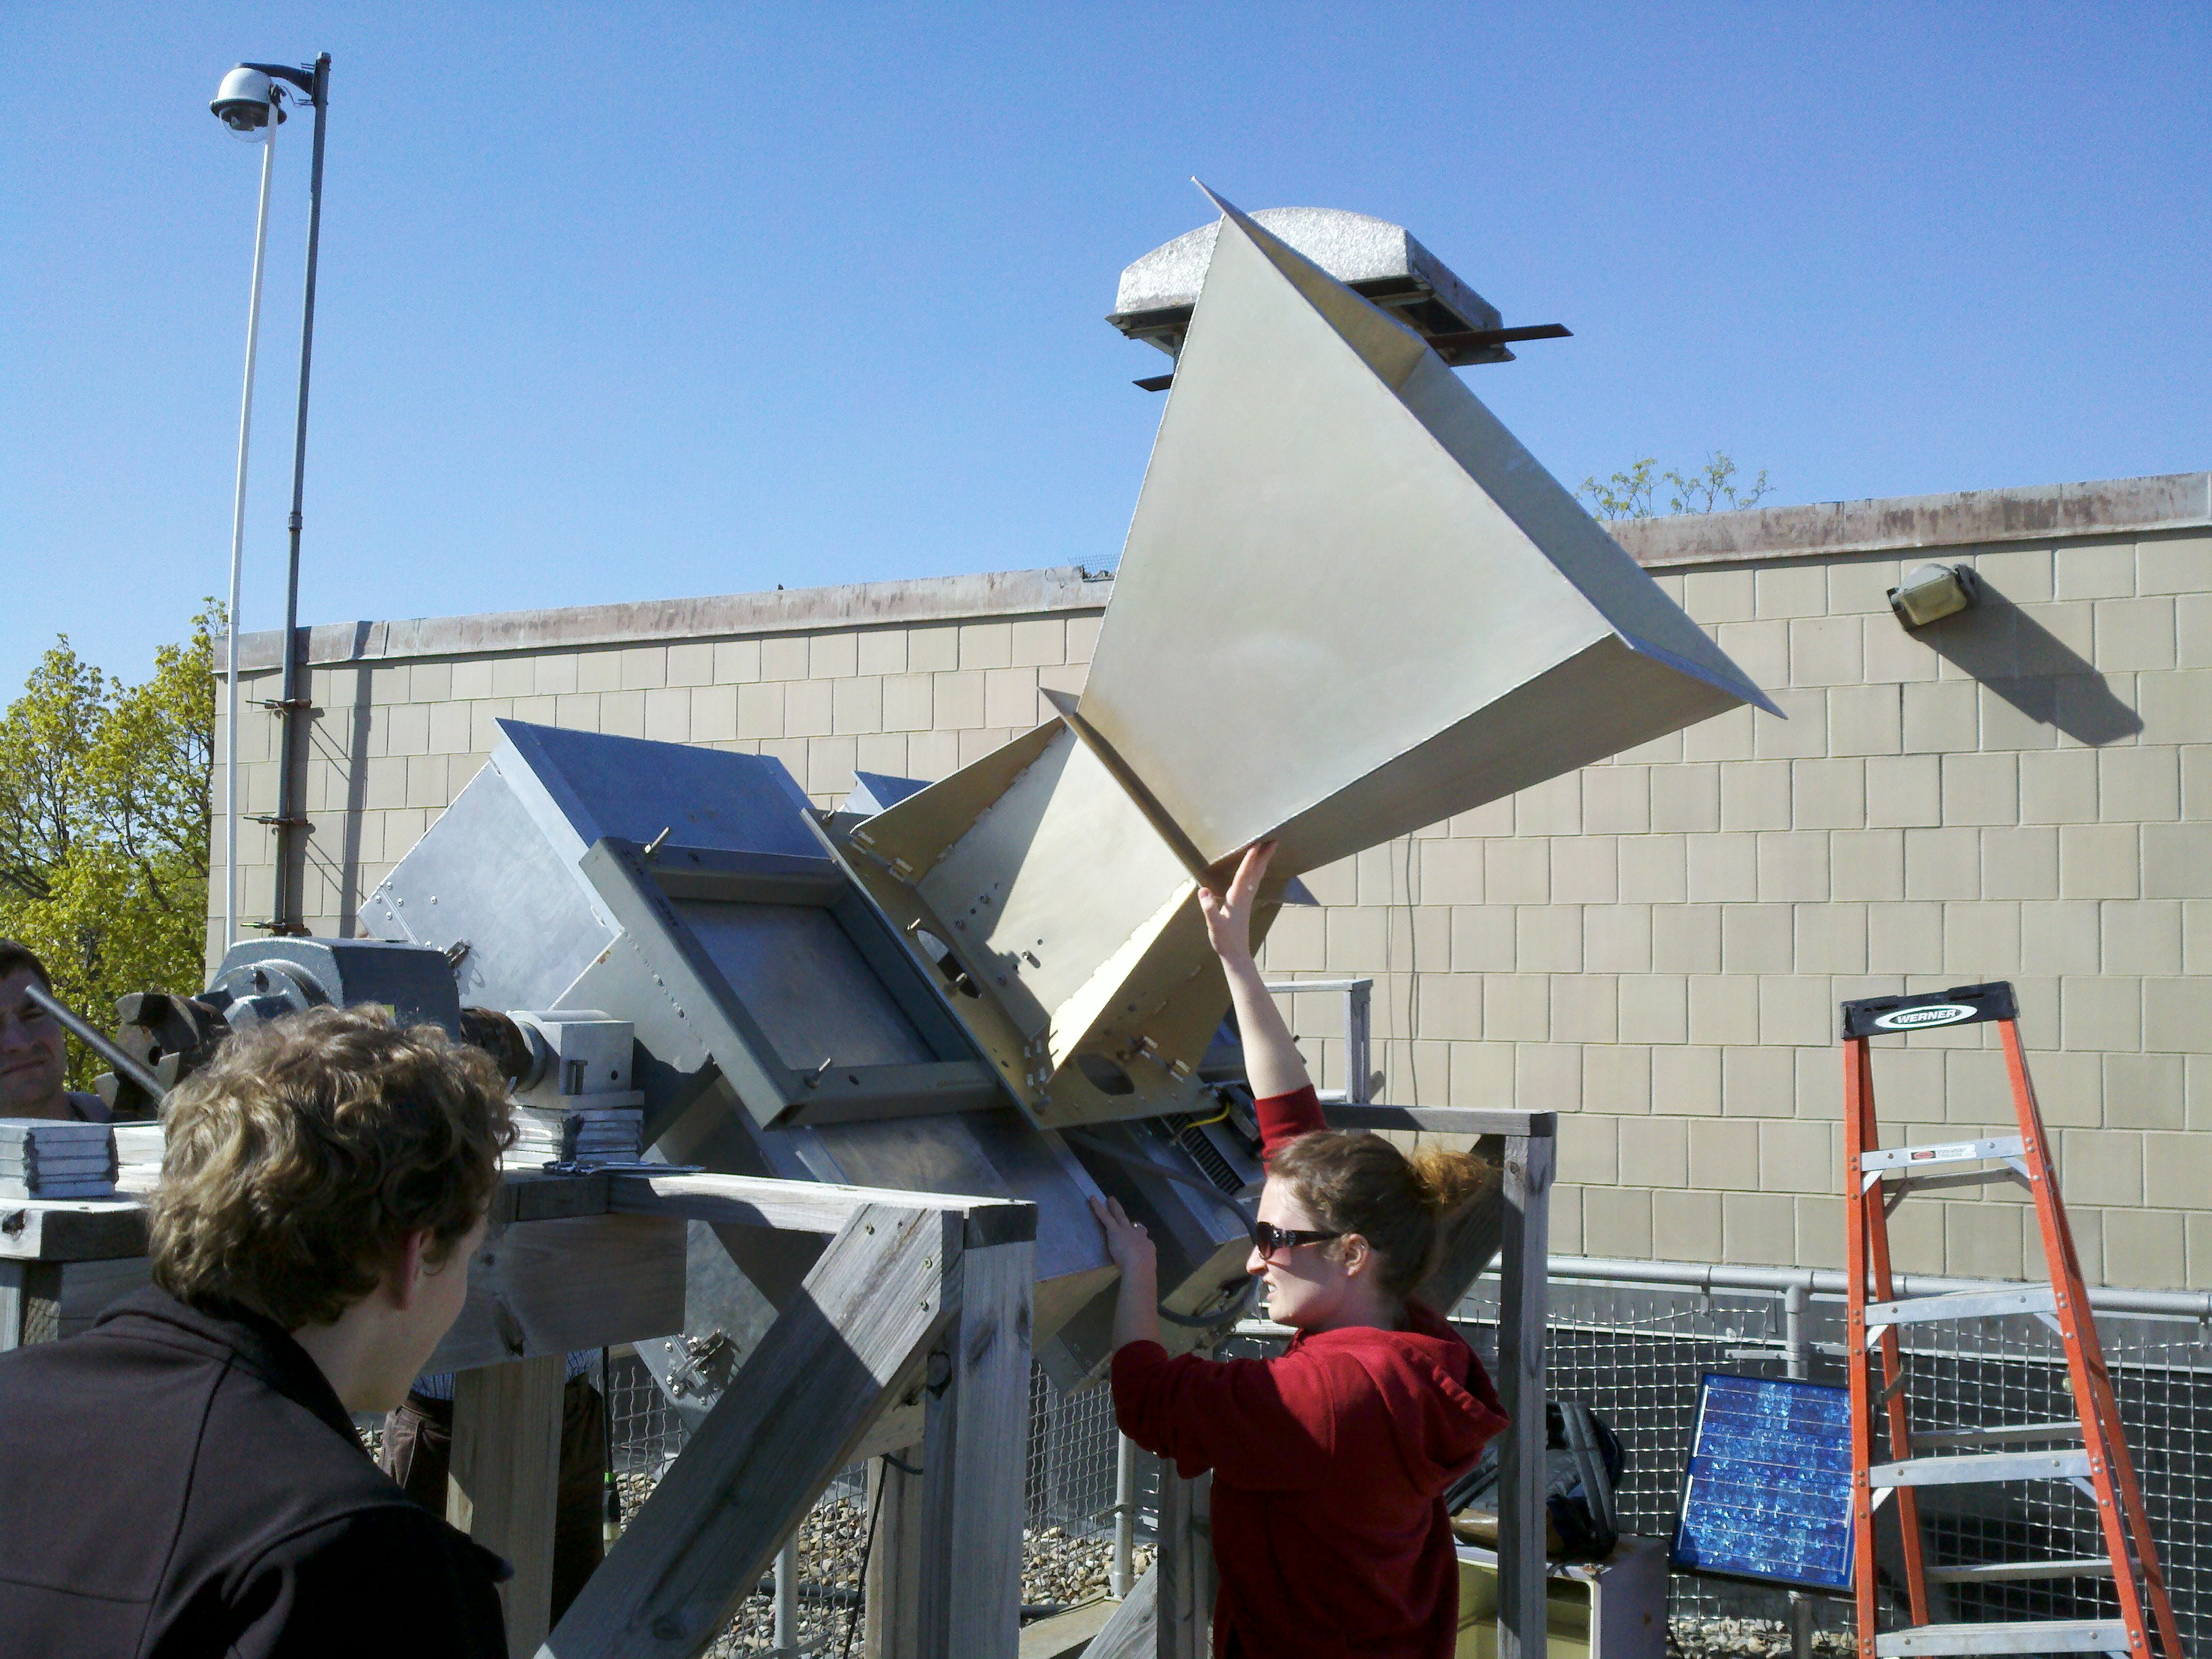
\includegraphics[width=\textwidth]{Images/radiometer_roof.jpg}
\isucaption{Students rotating the radiometer for an experiment on Agronomy Hall}
\label{radiometer_roof}
\end{figure}
}

The E E 518 test however showed that there were additional problems with the radiometer.  While the test showed that the SDR could in fact read data, the data was skewed.  It was later found out that the radiometer was generating an interfering signal that caused the power readings to be elevated.  That was found as a result of having the SDR record the signal and then was analyzed later.  Through this analysis, we found that a strong harmonic was developed and caused a spike in signal being recorded.  Although the exact reason for this has not been found, the problem has been isolated to something in the RF Front End of the ISU radiometer.  